Auf den Screenshots sieht man die eingebundene Schnittstelle. Die digitale Signatur kann als Unterschrift auf eine Verkaufsrechnung bzw. Vermietungsbeleg hinterlegt und ausgedruckt werden. 
\begin{figure}[!ht]
    \centering
    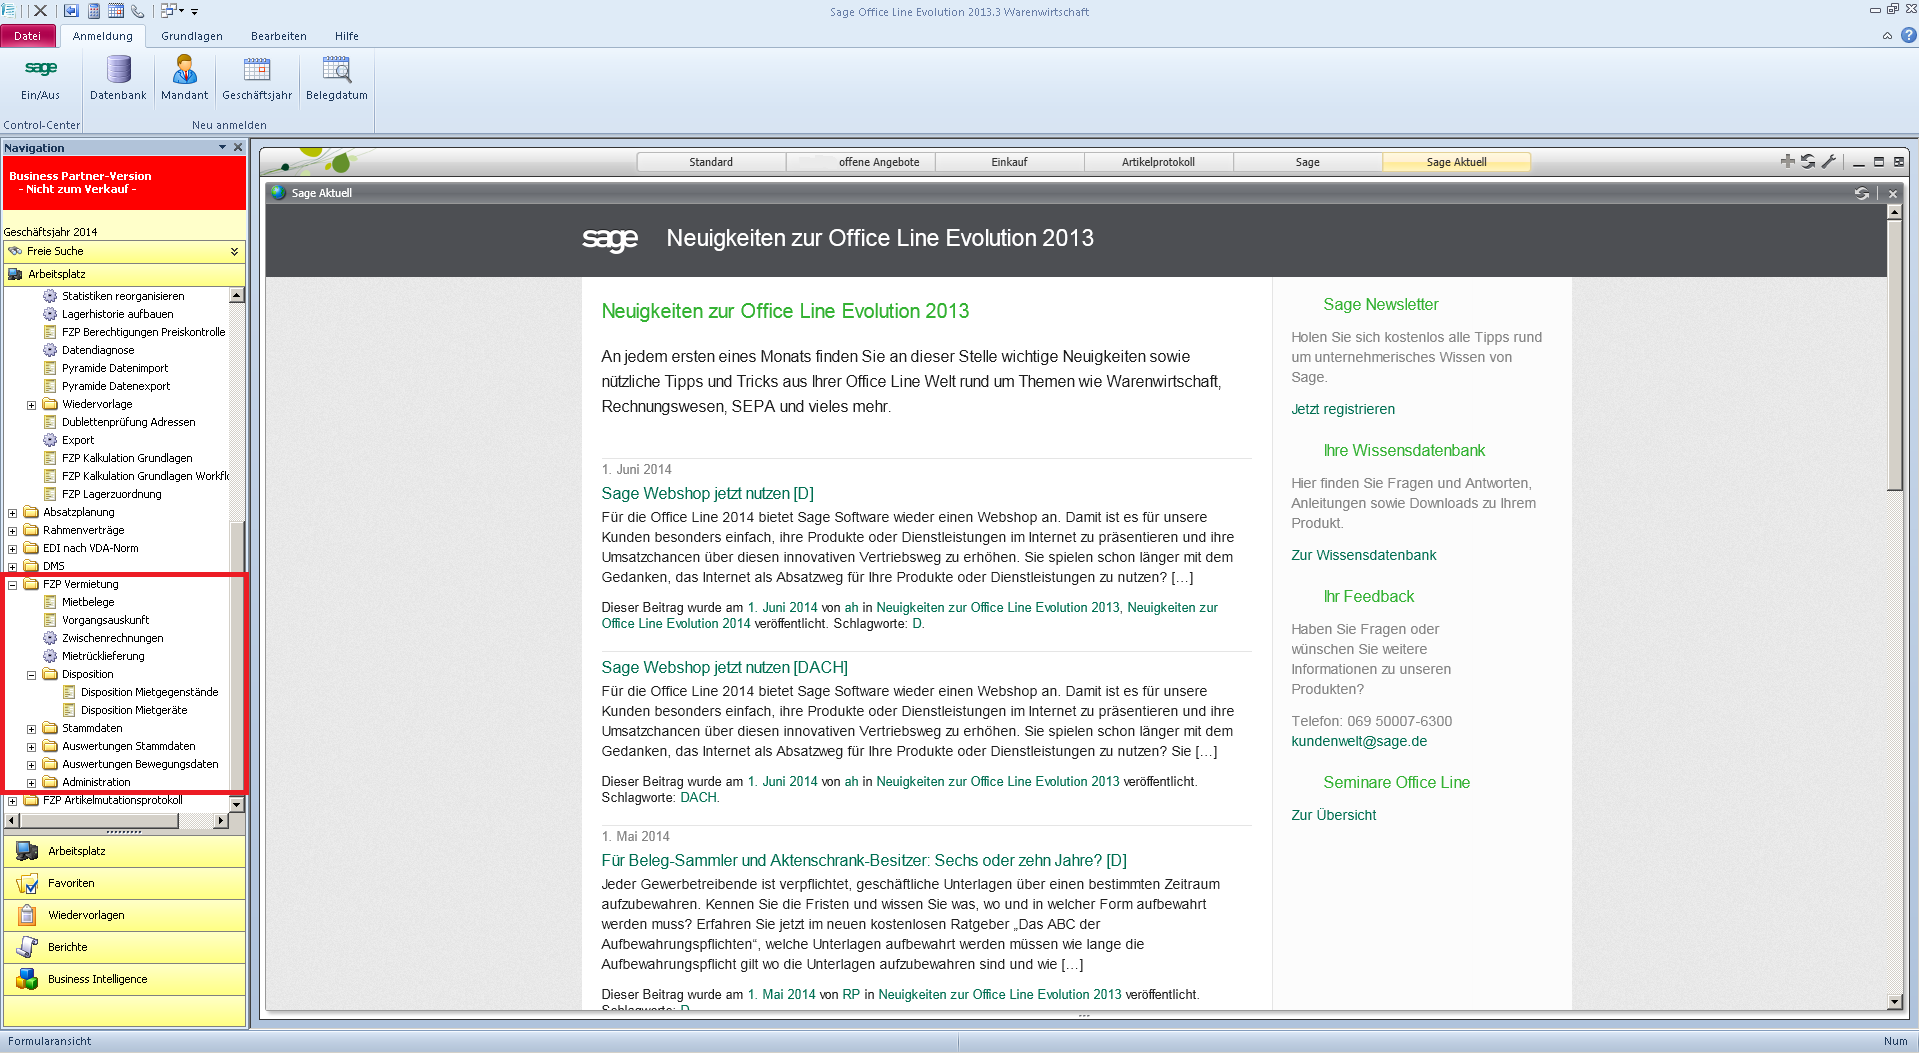
\includegraphics[height=250pt, width=450pt]{ol.PNG}
    \caption[Hauptansicht Sage Office Line]{Hauptansicht Sage Office Line}
\end{figure}\\
\begin{figure}[!ht]
    \centering
    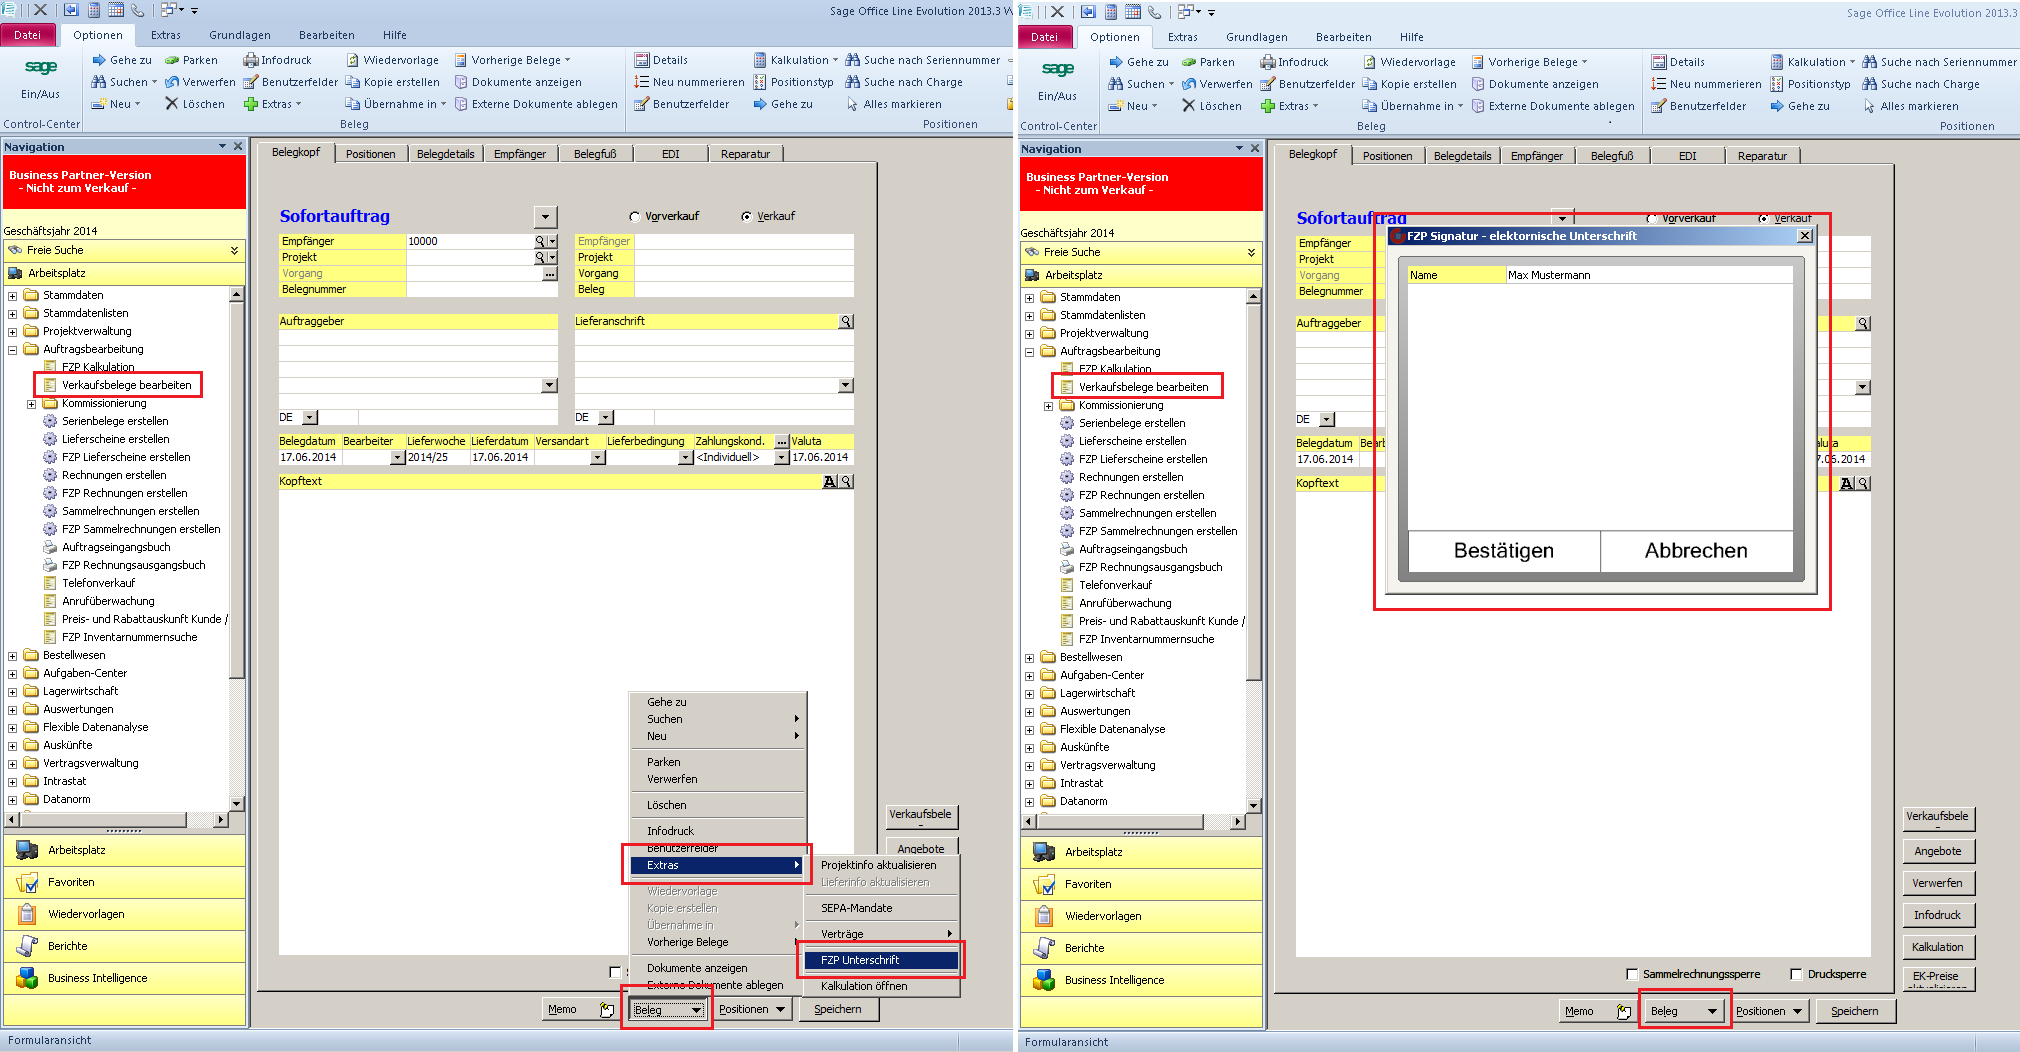
\includegraphics[height=250pt, width=450pt]{DigiSigVKBeleg3.png}
    \caption[Ablauf Erfassung digitale Signatur in Sage Office Line (Verkauf)]{Ablauf Erfassung digitale Signatur im Bereich Verkauf in Sage Office Line}
\end{figure}\\
\begin{figure}[!ht]
    \centering
    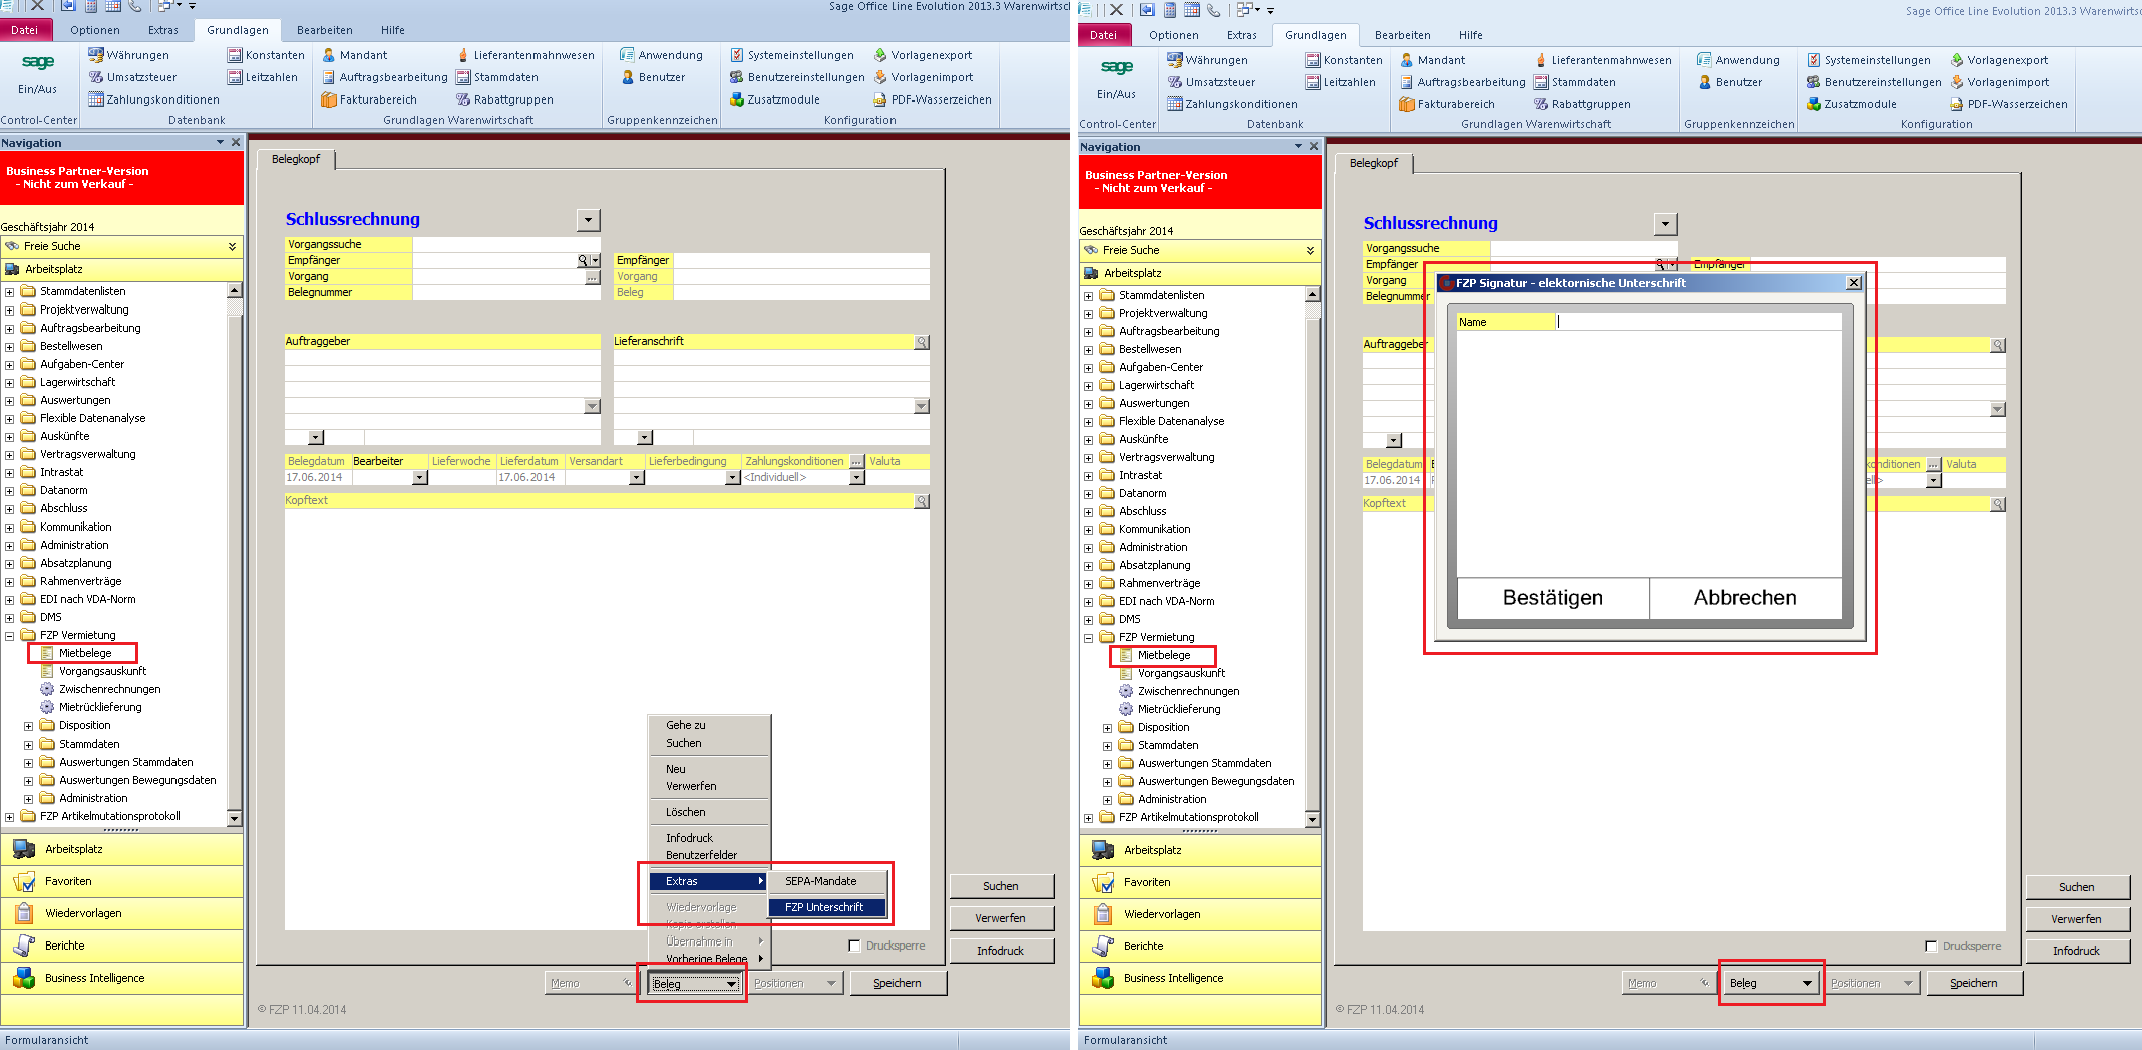
\includegraphics[height=250pt, width=450pt]{DigiSigVMBeleg3.png}
    \caption[Ablauf Erfassung digitale Signatur in Sage Office Line (Vermietung)]{Ablauf Erfassung digitale Signatur im Bereich Vermietung in Sage Office Line}
\end{figure}